% Prof. Dr. Ausberto S. Castro Vera
% UENF - CCT - LCMAT - Curso de Ci\^{e}ncia da Computa\c{c}\~{a}o
% Campos, RJ,  2022
% Disciplina: Paradigmas de Linguagens de Programa\c{c}\~{a}o
% Aluno: Ricardo Willian Pontes da Silva



\chapter{ Aplica\c{c}\~{o}es da Linguagem Python}

No capítulo a seguir serão apresentadas cinco aplica\c{c}\~{o}es completas na linguagem Python, contento:
\begin{itemize}
  \item Uma breve descri\c{c}\~{a}o da aplica\c{c}\~{a}o
  \item O c\'{o}digo completo da aplica\c{c}\~{a}o,
  \item Imagens do c\'{o}digo fonte no compilador-interpretador,
  \item Imagens dos resultados ap\'{o}s a compila\c{c}\~{a}o-interpreta\c{c}\~{a}o do c\'{o}digo fonte
  \item Links e referencias bibliogr\'{a}ficas de onde foi obtido a aplica\c{c}\~{a}o
\end{itemize}




    \section{Opera\c{c}\~{o}es b\'{a}sicas}


    \section{Programas gr\'{a}ficos}
A linguagem Python é altamente permissiva a manipulação de dados, e com isso existem ferramentas que se utilizam desse estudo de informações, como a criação de gráficos. Para isso é necessário a utilização da biblioteca Matplotlib que é basicamente uma ferramenta para criação de gráficos e visualização dos mesmos.

\begin{lstlisting}
import sys
import matplotlib
matplotlib.use('Agg')

import matplotlib.pyplot as plt
import numpy as np

x = np.array(["prova1","prova2","prova3","prova4"])
y = np.array([3, 8, 1, 10])

plt.plot(x, y)
plt.show()
plt.savefig(sys.stdout.buffer)
sys.stdout.flush()

	
\end{lstlisting}
  
  \begin{figure}[H]
  	\begin{center}
  		\caption{Gráfico gerado pela biblioteca matplotlib} \label{ling1}
  		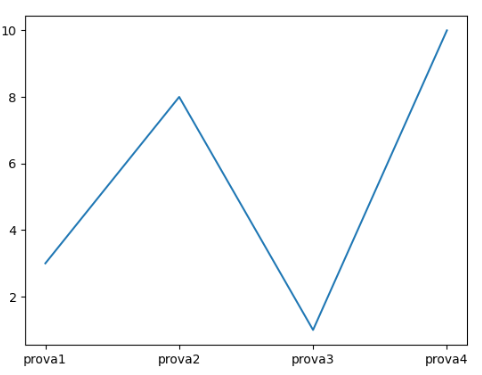
\includegraphics[width=9cm]{grafico py.PNG} \\
  		{\tiny \sf Fonte:{ Autor}}
  	\end{center}
  \end{figure}
  
    \section{Programas com Objetos}


    \section{O algoritmo Quicksort - Implementa\c{c}\~{a}o}


    \section{Aplica\c{c}\~{o}es com Banco de Dados}

